\documentclass[fontset=windows, 12pt]{article}
\usepackage{ctex}
\usepackage{pythontex}
\usepackage{graphicx}
\usepackage{float}

\title{Pythontex学习}
\author{Eureka}
\date{\today}

%% 注意:使用pythontex时可能会产生如下报错:
% Traceback (most recent call last):
%   File "c:\texlive\2021\texmf-dist\scripts\pythontex\pythontex.py", line 55, in <module>
%     import pythontex3 as pythontex
%   File "c:\texlive\2021\texmf-dist\scripts\pythontex\pythontex3.py", line 61, in <module>
%     from pygments.styles import get_all_styles
% ModuleNotFoundError: No module named 'pygments'

%% 解决方法:安装一个python的pygments包就行了
%% 执行命令:pip install pygments 

% 注:定义的python函数不能随意缩进,必须和下面相同
\begin{pycode}
def test():
    print("I am Pythontexm, Im Coming!")
    return ""
\end{pycode}
% 使用return ""是为了防止返回NONE,影响输出


\begin{document}
\maketitle
  \section{在LaTeX中使用Python}
  有了pythontex之后我们就可以在LaTeX中较为方便的使用python了,
  而没必要使用JinJia库来处理了。


  \subsection{在pycode环境中使用}
  % 注:这里也不能有任何的缩进。比如下面的代码就会报错
% \begin{pycode} 
%   print("Hello, it's me!")
% \end{pycode}

% 换行的原理和LaTeX相同
  \begin{pycode} 
print("Hello, I'm PythonTex!")
print("\n")
# 使用\n来换行
print("这是一段中文")
  \end{pycode}

  % 注:这里可以有缩进。
  \subsection{在py命令中使用}
  \py{print("测试py命令")}

   % 注:这里可以有缩进。
  \subsection{测试自定义函数}
  \py{test()}

  \newpage
  \subsection{测试循环}
  \begin{pycode}
for i in range(1,10):
  print("这是第"+str(i)+"句话")
  print("\n")
  \end{pycode}


  \subsection{测试绘制函数图像}
  % 生成图片:Tran.pdf
    \begin{pycode}
from matplotlib import pyplot as plt
import numpy as np

x = np.linspace(0, 2*np.pi, num = 80)
y = np.sin(x)
plt.plot(x, y)

plt.savefig("Tran.pdf")
    \end{pycode} 

  % 插入图片
  \begin{figure}[!htb]
     \centering
      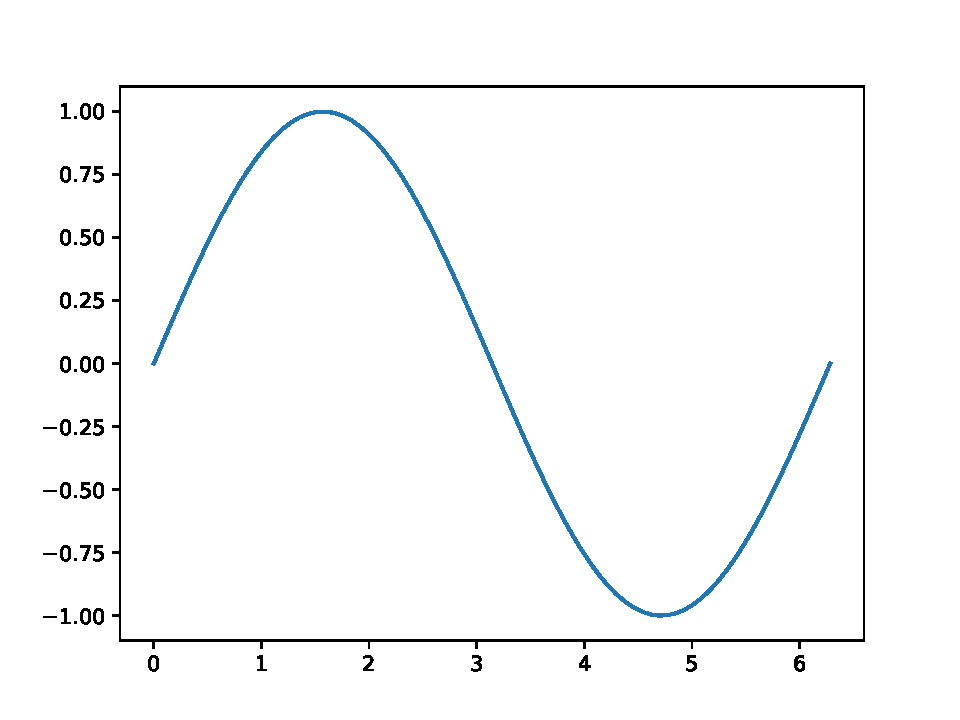
\includegraphics[scale=0.5]{Tran.pdf}
      \label{a}
      \caption{三角函数图像}
  \end{figure}


\end{document}
